%
%---Beginning of Document---
%
% Use 1). latex ftof_manual.tex, 2). dvipdfm ftof_manual
%
\documentclass[12pt]{article}
\usepackage[dvips]{color,graphics}
\usepackage{longtable}
\usepackage{hyperref}
\usepackage[pdftex]{graphicx}
\usepackage[absolute,overlay]{textpos}
\setlength{\TPHorizModule}{1mm}
\setlength{\TPVertModule}{1mm}
%
\textwidth  6.5in
\textheight 9.0in
\topmargin 0.0 in
\headheight 0.0in
\headsep 0.0in
\oddsidemargin 0in
\evensidemargin 0in
\parsep 0 in
%\parindent 0in
\pagenumbering{arabic}
%
\setcounter{secnumdepth}{5}
\setcounter{tocdepth}{5}
%
\begin{document}

\title{Forward Time-of-Flight System Operations Manual}

\vskip 0.5cm

\author{D.S. Carman, Jefferson Laboratory\\[0.2ex]
{\it ftof\_manual.tex -- v2.0}}

\date \today
%
\maketitle

\begin{abstract}
This document provides an overview of the CLAS12 Forward Time-of-Flight (FTOF) System 
and serves as an Operations Manual for the detector. Instructions are provided for 
shift workers related to the basic steps of operating and monitoring the HV controls, 
monitoring the detector system and responding to alarms, and knowing when to contact 
the on-call personnel. More complete details are also provided for FTOF system experts 
regarding the channel mapping to the readout electronics, the cable connections and 
routing in Hall~B, higher-order high voltage system operations, and detector servicing. 
This document also provides references to the available FTOF documentation and a list 
of personnel authorized to perform FTOF system repairs and to modify system settings.
\end{abstract}

\thispagestyle{empty}

\clearpage

\vfil
\eject

\tableofcontents

\vfil
\eject

\section{FTOF Overview}
\label{intro}

The Forward Time-of-Flight (FTOF) system is a major component of the CLAS12 Forward 
Detector that is used to measure the flight time of charged particles emerging from 
beam-related interactions in the target. The average path length from the target to 
the FTOF counters is roughly 6 - 7~m. The system requirements include excellent timing 
resolution for particle identification and good segmentation to provide for flexible 
triggering options. The system specifications call for an average time resolution of 
$\sigma_{TOF}$=80~ps at the more forward angles of CLAS12 ($\theta < 35^\circ$) and 
150~ps at larger angles ($\theta > 35^\circ$). The system must also be capable of 
operating in a high-rate environment. At the nominal CLAS12 operating luminosity of 
$1 \times 10^{35}$~cm$^{-2}$s$^{-1}$, the average rate per scintillation counter approaches
1~MHz.

%%%%%%%%%%%%%%%%%%%%%%%%%%%%%%%%%%%%%%%%%%%%%%%%%%%%%%%
\begin{figure}[htbp]
\vspace{4.8cm}
\begin{picture}(50,50) 
\put(130,-33)
{\hbox{\includegraphics[width=0.40\textwidth,natwidth=610,natheight=642]{fwd_car.pdf}}}
\end{picture} 
\caption{View of the FTOF for CLAS12 highlighting the location of the counters. The panel-1b
arrays are shown in blue and the panel-2 arrays, mounted around the perimeter of the Forward
Carriage, are shown in orange. The panel-1a arrays are mounted immediately downstream of the
panel-1b arrays, and are not visible in this picture. The Forward Carriage is roughly 10~m in
diameter.} 
\label{fwd_car}
\end{figure}
%%%%%%%%%%%%%%%%%%%%%%%%%%%%%%%%%%%%%%%%%%%%%%%%%%%%%%%

The CLAS12 spectrometer in the forward direction is built around a six-coil superconducting
toroidal magnet that divides the active detection area into six 60$^\circ$-wide azimuthal
regions called sectors. In each of the six sectors of the CLAS12 Forward Detector, the FTOF
system is comprised of three arrays of counters, referred to as panels, named panel-1a,
panel-1b, and panel-2.  Each panel consists of a set of rectangular scintillators with a PMT on
each end.  Panel-1 includes the sets of counters located at forward angles (roughly 5$^\circ$ to 
35$^\circ$) and panel-2 includes the sets of counters at larger angles (roughly $35^\circ$ to 
45$^\circ$). The positioning and attachment of the FTOF detector arrays on the Forward Carriage 
of CLAS12 are shown in Fig.~\ref{fwd_car}. Each of the six panel-1a arrays contains 23 counters, 
each of the six panel-1b arrays contains 62 counters, and each of the six panel-2 arrays contains 
5 counters.

Figure~\ref{ftof-naming} shows the sector naming and identifier conventions for the FTOF 
system, as well as the definitions of the left and right sides of each sector. A summary 
of the FTOF technical parameters is given in Table~\ref{details}. 

%%%%%%%%%%%%%%%%%%%%%%%%%%%%%%%%%%%%%%%%%%%%%%%%%%%%%%%
\begin{figure}[htbp]
\vspace{8.0cm}
\begin{picture}(30,50) 
\put(90,0)
{\hbox{\includegraphics[width=1.0\textwidth,natwidth=610,natheight=642]{ftof-naming.pdf}}}
\end{picture} 
\caption{Schematic view of the Hall B Forward Carriage looking downstream along the 
electron beamline showing the sector naming convention, the definitions of the left (L) 
and right (R) sides of each sector, and the clock position identifier. The electron 
beam goes into the page such that S1 is on beam left and S4 is on beam right.}
\label{ftof-naming}
\end{figure}
%%%%%%%%%%%%%%%%%%%%%%%%%%%%%%%%%%%%%%%%%%%%%%%%%%%%%%%

%%%%%%%%%%%%%%%%%%%%%%%%%%%%%%%%%%%%%%%%%%%%%%%%%%%%%%%
\begin{table}[ht]
\begin{center}
\begin{tabular} {|c|l|} \hline
~~Parameter~~ &~~~~~~~~~~~~~~~~~~~~~~ Design Value ~~~~~~~~~~\\ \hline \hline
\multicolumn{2}{|l|} {\bf Panel-1a} \\ \hline
Angular Coverage      & $\theta = 5^\circ \to 35^\circ$, $\phi: 50\% {\rm ~at~} 5^\circ \to 
85\% {\rm ~at~} 35^\circ$ \\ \hline
Counter Dimensions    & $L = 32.3$~cm $\to$ 376.1~cm, $w \times h$ = 15~cm $\times$ 
5~cm \\ \hline
Scintillator Material & BC-408   \\ \hline
PMTs                  & EMI 9954A, Philips P2262 \\ \hline
Design Resolution     & 90~ps $\to$ 160~ps   \\ \hline \hline
\multicolumn{2}{|l|} {\bf Panel-1b} \\ \hline
Angular Coverage      & $\theta = 5^\circ \to 35^\circ$, $\phi: 50\% {\rm ~at~} 5^\circ \to 
85\% {\rm ~at~} 35^\circ$ \\ \hline
Counter Dimensions    & $L = 17.3$~cm $\to$ 407.9~cm, $w \times h$ = 6~cm $\times$ 6~cm  
\\ \hline
Scintillator Material & BC-404 (\#1 $\to$ \#31), BC-408 (\#32 $\to$ \#62)  \\ \hline
PMTs                  & Hamamatsu R9779 \\ \hline
Design Resolution     & 60~ps $\to$ 110~ps   \\ \hline \hline
\multicolumn{2}{|l|} {\bf Panel-2} \\ \hline
Angular Coverage      & $\theta = 35^\circ \to 45^\circ$, $\phi: 85\% {\rm ~at~} 35^\circ \to 
95\% {\rm ~at~} 45^\circ$ \\ \hline
Counter Dimensions    & $L = 371.3$~cm $\to$ 426.1~cm, $w \times h$ = 22~cm $\times$ 
5~cm \\ \hline
Scintillator Material & BC-408   \\ \hline
PMTs                  & Photonis XP4312B, EMI 4312KB \\ \hline
Design Resolution     & 145~ps $\to$ 160~ps   \\ \hline
\end{tabular}
\caption{Table of parameters for the scintillation bars, PMTs, and counters for the 
FTOF panel-1a, panel-1b, and panel-2 arrays.}
\label{details}
\end{center}
\end{table}
%%%%%%%%%%%%%%%%%%%%%%%%%%%%%%%%%%%%%%%%%%%%%%%%%%%%%%%

%%%%%%%%%%%%%%%%%%%%%%%%%%%%%%%%%%%%%%%%%%%%%%%%%%%%%%%
\begin{figure}[htbp]
\vspace{5.8cm}
\begin{picture}(30,50) 
\put(95,200)
{\hbox{\includegraphics[width=0.85\textwidth,natwidth=610,natheight=642,angle=-90]
{electronics-block.pdf}}}
\end{picture} 
\caption{Block diagram for the FTOF system showing the layout of the readout electronics 
and HV connections for a single representative counter.}
\label{ftof-elec}
\end{figure}
%%%%%%%%%%%%%%%%%%%%%%%%%%%%%%%%%%%%%%%%%%%%%%%%%%%%%%%

A block diagram of the readout electronics for one counter of the FTOF system is shown 
in Fig.~\ref{ftof-elec}. The PMT anode outputs are connected to JLab VME leading edge 
discriminators and CAEN VME TDCs. Both high resolution TDCs (25~ps LSB CAEN 1290A) and 
lower resolution TDCs (100~ps LSB CAEN 1190A) are employed, where the lower resolution 
TDCs are associated with the longer counters at large polar angles for panel-1a, panel-1b, and
panel-2. The PMT dynode outputs are connected to JLab 250~MHz VME flash ADCs.  

The electronics for each sector are located behind the detectors on the three levels of the
Forward Carriage as follows:

\vskip 0.5cm

\begin{minipage}{0.5\textwidth}
\begin{itemize}
\item FTOF S1: FC Level 2 South
\item FTOF S2: FC Level 3 South
\item FTOF S3: FC Level 3 North
\end{itemize}
\end{minipage}
\begin{minipage}{0.5\textwidth}
\begin{itemize}
\item FTOF S4: FC Level 2 North
\item FTOF S5: FC Level 1 North
\item FTOF S6: FC Level 1 South
\end{itemize}
\end{minipage}

\vskip 0.5cm

Note that ``South'' refers to beam left and ``North'' to beam right (closer to the Pie 
Tower). Figure~\ref{fc-layout} shows the rack locations for the FTOF VME electronics and 
signal cable patch panels. 

The high voltage (HV) power supplies for each FTOF sector are either CAEN 1527LC 
mainframes or CAEN 4527 mainframes outfitted with negative polarity 24-channel A1535N 
modules. The HV mainframes that power the FTOF system are actually shared between the 
FTOF and the PCAL. The FTOF boards occupy slots \#0 to \#7 of each mainframe and the 
PCAL boards occupy slots \#8 to \#15 of each mainframe. The supplies are named HVFTOFn, 
n=1$\to$6 ({\it i.e.} HVFTOF1 $\to$ HVFTOF6). Figure~\ref{fc-layout} shows the locations 
of the HV mainframes for each of the FTOF sectors on the Forward Carriage.

%%%%%%%%%%%%%%%%%%%%%%%%%%%%%%%%%%%%%%%%%%%%%%%%%%%%%%%
\begin{figure}[htbp]
\vspace{12.0cm}
\begin{picture}(30,50) 
\put(35,375)
{\hbox{\includegraphics[width=0.65\textwidth,natwidth=610,natheight=642,angle=-90]
{fc-layout1.pdf}}}
\put(155,65)
{\hbox{\includegraphics[width=0.65\textwidth,natwidth=610,natheight=642,angle=-90]
{fc-layout2.pdf}}}
\put(425,340)
{\hbox{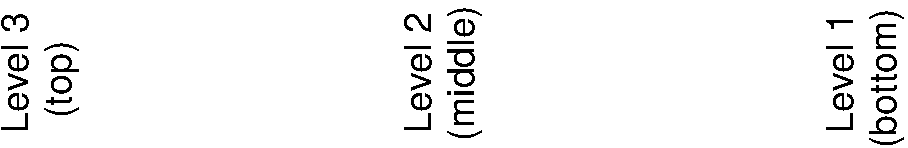
\includegraphics[width=0.65\textwidth,natwidth=610,natheight=642,angle=-90]
{fc-layout3.pdf}}}
\end{picture} 
\caption{Forward Carriage layout of the FTOF VME electronics, signal cable patch panels, 
and HV power supplies in the electronics racks on each of the three levels. The rack 
names on each level (c1, c2, and c3) are numbered 1 through 10. This view is looking 
upstream. Note: The racks on Level~1 are 180~cm tall and those for Levels~2 and 3 are 
210~cm tall. For this reason, the dynode patch panels are split into two neighboring
racks on Level~1.}
\label{fc-layout}
\end{figure}
%%%%%%%%%%%%%%%%%%%%%%%%%%%%%%%%%%%%%%%%%%%%%%%%%%%%%%%

\clearpage

\vfil
\eject

\section{Information for Shift Workers}

\subsection{Shift Worker Responsibilities}

The shift worker in the Hall~B Counting House has five responsibilities with regard to 
the FTOF system:

\begin{enumerate}
\item Updating the Hall~B electronic logbook with records of problems or system 
conditions (see Section~\ref{logbook});

\item Contacting FTOF system on-call personnel for any problems that are discovered 
(see Section~\ref{contact});

\item Responding to FTOF system alarms from the Hall~B alarm handler (see 
Section~\ref{alarms});

\item Turning on or off the high voltage for the FTOF system using the HV control 
interface (see Section~\ref{hv-control});

\item Monitoring the hit occupancy scalers for the system (see Section~\ref{monitoring}).
\end{enumerate}

\subsubsection{Updating the Logbook}
\label{logbook}

The electronic logbook (or e-log)~\cite{e-log} is set up to run on a specified terminal 
in the Hall~B Counting House. Shift workers are responsible for keeping an up-to-date 
and accurate record of any problems or issues concerning the FTOF system. For any 
questions regarding the logbook, its usage, or on what is considered to be a ``logbook 
worthy'' entry, consult the assigned shift leader.

Note the shift worker should follow all posted or communicated instructions about entering 
FTOF monitoring histograms into the e-log. This is typically done (at least) once per 8-hour 
shift as directed on the shift checklist.

\subsubsection{Contacting FTOF System Personnel}
\label{contact}

As a general rule, shift workers should spend no more than 10 to 15 minutes attempting to 
solve any problem that arises with the FTOF system. At that point they should contact the 
assigned FTOF on-call expert either to provide advice on how to proceed or to address the 
problem. \textcolor{red}{The FTOF on-call phone number is (757)-344-7204.}

This document is divided into sections for shift workers and for FTOF system experts. 
However, only FTOF system experts (as listed in Section~\ref{personnel}) are authorized 
to make changes to the FTOF parameter settings, to work on the hardware or electronics, 
or to modify the data acquisition (DAQ) system settings. This division between shift worker
responsibilities and expert responsibilities is essential to maintain in order to protect
and safeguard the equipment, to ensure data collection is as efficient as possible, and to
minimize down time. If the shift worker has any questions regarding how to proceed when an
issue arises, the shift leader should be consulted.

\subsubsection{Hall~B Alarm Handler}
\label{alarms}

The BEAST alarm handler system running in the Counting House monitors the entire 
Hall~B Slow Controls system. This includes the HV and low voltage (LV) systems, gas 
systems, torus and solenoid controls, subsystem environment controls ({\it e.g.}
temperature, humidity), and pulser calibration systems (among several others). The system
runs on a dedicated terminal in the Counting House. One of the main responsibilities of the
shift worker is to respond to alarms from this system, either by taking corrective action
or by contacting the appropriate on-call personnel. Instructions and details on the alarm 
handler for Hall~B are given in Ref.~\cite{beast}.

The only element of the FTOF system monitored by the alarm handler is the HV system. 
Any time a channel trips off an alarm will sound. The alarm handler will identify the 
specific channel (or channels) that have tripped. These channels can be reset either 
through the alarm handler or through the nominal FTOF HV control screens. These channels 
should be reset only after ensuring that whatever condition caused the trip ({\it e.g.}
bad beam conditions) has been addressed.

\subsection{High Voltage Controls}
\label{hv-control}

The FTOF HV is controlled through the Hall~B CS-Studio suite, which is an Eclipse-based 
collection of tools used as an interface to the EPICS Slow Controls system. To start the 
user interface on any terminal in the Hall~B Counting House, enter the command ``clascss''.
Figure~\ref{ftof-screen1-2}(left) shows the control panel that is launched.

%%%%%%%%%%%%%%%%%%%%%%%%%%%%%%%%%%%%%%%%%%%%%%%%%%%%%%%
\begin{figure}[htbp]
\vspace{8.5cm}
\begin{picture}(30,50) 
\put(40,-5)
{\hbox{\includegraphics[width=0.50\textwidth,natwidth=610,natheight=642]
{ftof-hv-screen-1.pdf}}}
\put(190,-5)
{\hbox{\includegraphics[width=0.50\textwidth,natwidth=610,natheight=642]
{ftof-hv-screen-2.pdf}}}
\end{picture} 
\caption{The CS-Studio interface used for the Slow Controls of the CLAS12 detectors and
subsystems. (Left) General CLAS12 interface. (Right) Options for the FTOF system.}
\label{ftof-screen1-2}
\end{figure}
%%%%%%%%%%%%%%%%%%%%%%%%%%%%%%%%%%%%%%%%%%%%%%%%%%%%%%%

To bring up the FTOF HV controls, click on the ``FTOF'' button on the subsystem list. 
This pops up a sub-menu of all Slow Controls subprograms for the FTOF system (see 
Fig.~\ref{ftof-screen1-2}(right)). Clicking the mouse on the ``FTOF HV'' option brings 
up the HV control interface for the FTOF system as shown in Fig.~\ref{ftof-screen3}. 
This interface allows for HV operations at a number of functionality levels:

\begin{itemize}
\item All channels in the full FTOF system
\item All channels in a single FTOF sector (panel-1a, panel-1b, panel-2)
\item All channels in a single sector for a given panel
\item A single PMT in the FTOF system
\end{itemize}

%%%%%%%%%%%%%%%%%%%%%%%%%%%%%%%%%%%%%%%%%%%%%%%%%%%%%%%
\begin{figure}[htbp]
\vspace{6.5cm}
\begin{picture}(30,50) 
\put(80,235)
{\hbox{\includegraphics[width=0.50\textwidth,natwidth=610,natheight=642,angle=-90]
{ftof-hv-screen-3.pdf}}}
\end{picture} 
\caption{FTOF HV display and control interface.}
\label{ftof-screen3}
\end{figure}
%%%%%%%%%%%%%%%%%%%%%%%%%%%%%%%%%%%%%%%%%%%%%%%%%%%%%%%

The HV Control Interface screen (see Fig.~\ref{ftof-screen3}) also provides a color key 
to indicate the channel status:

\begin{itemize}
\item HV off - no highlight color (channel color dark green)
\item HV on - bright green
\item HV ramping up or ramping down - orange
\item HV trip - red
\item Communication problem - yellow
\item Undefined channel status - magenta
\end{itemize}

For the shift worker the most common operations are:

\begin{enumerate}
\item To turn the HV for all system PMTs on or off. This is accomplished by clicking 
the button in the upper right corner ``ALL ON/OFF''. This pops up a sub-menu with the 
relevant options ``Turn All Off'' and ``Turn All On''.
\item To turn individual PMTs on or off. This is accomplished by clicking on the circle 
representing the channel of interest. This brings up a control screen for the channel of 
interest as shown in Fig.~\ref{ftof-screen4}. Clicking on the button in the ``Pw'' (Power)
column toggles the channel HV on and off.
\item To turn the HV for all PMTs in a single sector on or off. This is accomplished 
by clicking on the sector button in the upper right corner (S1 $\to$ S6) (see 
Fig.~\ref{ftof-screen3}). This pops up a sub-menu with the relevant options ``Turn Sector XX
Off'' and ``Turn Sector XX On''.
\item To turn the HV for all PMTs in a given panel and sector on or off. This is 
accomplished by clicking on the Sector button (Sector~1 $\to$ Sector~6) next to the 
panel of interest. This pops up a sub-menu with the relevant options as shown in 
Fig.~\ref{ftof-screen5}.
\end{enumerate}

%%%%%%%%%%%%%%%%%%%%%%%%%%%%%%%%%%%%%%%%%%%%%%%%%%%%%%%
\begin{figure}[htbp]
\vspace{0.5cm}
\begin{picture}(30,50) 
\put(85,150)
{\hbox{\includegraphics[width=0.50\textwidth,natwidth=610,natheight=642,angle=-90]
{ftof-hv-screen-4.pdf}}}
\end{picture} 
\caption{FTOF HV display for single channel parameters.}
\label{ftof-screen4}
\end{figure}
%%%%%%%%%%%%%%%%%%%%%%%%%%%%%%%%%%%%%%%%%%%%%%%%%%%%%%%

%%%%%%%%%%%%%%%%%%%%%%%%%%%%%%%%%%%%%%%%%%%%%%%%%%%%%%%
\begin{figure}[htbp]
\vspace{5.8cm}
\begin{picture}(30,50) 
\put(85,230)
{\hbox{\includegraphics[width=0.50\textwidth,natwidth=610,natheight=642,angle=-90]
{ftof-hv-screen-5.pdf}}}
\end{picture} 
\caption{FTOF HV display and control interface to open channel controls for a given panel 
and sector.}
\label{ftof-screen5}
\end{figure}
%%%%%%%%%%%%%%%%%%%%%%%%%%%%%%%%%%%%%%%%%%%%%%%%%%%%%%%

Note that hovering the mouse pointer on  a circle representing a PMT brings up EPICS
information on that channel as shown in Fig.~\ref{ftof-screen3a}.

%%%%%%%%%%%%%%%%%%%%%%%%%%%%%%%%%%%%%%%%%%%%%%%%%%%%%%%
\begin{figure}[htbp]
\vspace{6.5cm}
\begin{picture}(30,50) 
\put(85,230)
{\hbox{\includegraphics[width=0.50\textwidth,natwidth=610,natheight=642,angle=-90]
{ftof-hv-screen-3a.pdf}}}
\end{picture} 
\caption{FTOF HV display showing the channel information when the mouse is paused over a 
PMT circle.}
\label{ftof-screen3a}
\end{figure}
%%%%%%%%%%%%%%%%%%%%%%%%%%%%%%%%%%%%%%%%%%%%%%%%%%%%%%%

If the ``Open Channel Controls'' option shown in Fig.~\ref{ftof-screen5} is selected, a 
``novice'' window is opened as shown in Fig.~\ref{ftof-screen6}. This window shows the 
monitored channel voltages and currents ($V_{mon}$ (V) and $I_{mon}$ ($\mu$A)), the channel 
statuses (OFF, ON), and the set channel voltages and currents ($V_{set}$ (V) and $I_{set}$ 
($\mu$A)). If desired, shift workers can toggle the HV settings for single channels on 
or off through this interface.

%%%%%%%%%%%%%%%%%%%%%%%%%%%%%%%%%%%%%%%%%%%%%%%%%%%%%%%
\begin{figure}[htbp]
\vspace{9.0cm}
\begin{picture}(30,50) 
\put(105,-15)
{\hbox{\includegraphics[width=0.55\textwidth,natwidth=610,natheight=642]
{ftof-hv-screen-6.pdf}}}
\end{picture} 
\caption{FTOF ``novice'' channel controls screen.}
\label{ftof-screen6}
\end{figure}
%%%%%%%%%%%%%%%%%%%%%%%%%%%%%%%%%%%%%%%%%%%%%%%%%%%%%%%

In the upper left corner of this ``Channel Controls'' window is a button marked 
``expert'' that brings up the window shown in Fig.~\ref{ftof-screen7}. This allows 
changes to the system settings for the maximum channel current, maximum channel 
voltage setting, and the channel HV ramp up and ramp down rates. Clicking on the 
``novice'' button in the upper left corner toggles between the expert and novice 
screens. \textcolor{red}{The expert screen should only be used by the list of 
authorized FTOF personnel given in Section~\ref{personnel}.} 

%%%%%%%%%%%%%%%%%%%%%%%%%%%%%%%%%%%%%%%%%%%%%%%%%%%%%%%
\begin{figure}[htbp]
\vspace{7.5cm}
\begin{picture}(30,50) 
\put(60,265)
{\hbox{\includegraphics[width=0.57\textwidth,natwidth=610,natheight=642,angle=-90]
{ftof-hv-screen-7.pdf}}}
\end{picture} 
\caption{FTOF ``expert'' channel controls screen.}
\label{ftof-screen7}
\end{figure}
%%%%%%%%%%%%%%%%%%%%%%%%%%%%%%%%%%%%%%%%%%%%%%%%%%%%%%%

\subsubsection{Resetting the IOCs}
\label{reset-iocs}

If there is a controls problem indicated by the appearance of yellow or magenta channels
in Fig.~\ref{ftof-screen3}, which typically appears for all PMTs in a given sector, the
usual cause is an issue of communication between the IOC computer and the HV mainframe.
To reboot the IOC for a given sector, click on the ``IOCs'' button on the Slow Controls
panel within the ``Subsystems'' portion of the interface. Figure~\ref{ioc-reset2} shows the
options that appear on the sub-menu that pops up. On this menu, select ``IOC Health'' to
open the control window shown in Fig.~\ref{ioc-reset3}. Clicking on the ``High Voltage''
tab along the top of the screen brings up the screen for the IOCs that control the HV
mainframes as shown in Fig.~\ref{ioc-reset4}. Click on the ``Reboot'' button (under the
``Soft Reboot'' column) for the HV supply that has the IOC communication problem. The
reboot will take less than two minutes to complete and the yellow or magenta communication
problem channel indicators should all disappear. Note that the IOCs can be also rebooted
through the FTOF channel control screen shown in Fig.~\ref{ftof-screen3}. Click on the
``IOCs'' button in the upper left corner and then click on the ``Reboot'' button for the
sector of interest. If rebooting the IOC does not solve the problems, contact the Slow
Controls system expert.

%%%%%%%%%%%%%%%%%%%%%%%%%%%%%%%%%%%%%%%%%%%%%%%%%%%%%%%
\begin{figure}[htbp]
\vspace{9.0cm}
\begin{picture}(30,50) 
\put(125,0)
{\hbox{\includegraphics[width=0.50\textwidth,natwidth=610,natheight=642]{ioc-reset2.pdf}}}
\end{picture} 
\caption{Sub-menu on the primary Slow Controls interface to reboot the IOCs.}
\label{ioc-reset2}
\end{figure}
%%%%%%%%%%%%%%%%%%%%%%%%%%%%%%%%%%%%%%%%%%%%%%%%%%%%%%%

%%%%%%%%%%%%%%%%%%%%%%%%%%%%%%%%%%%%%%%%%%%%%%%%%%%%%%%
\begin{figure}[htbp]
\vspace{5.0cm}
\begin{picture}(30,50) 
\put(10,265)
{\hbox{\includegraphics[width=0.75\textwidth,natwidth=610,natheight=642,angle=-90]
{ioc-reset3.pdf}}}
\end{picture} 
\caption{IOC health screen for access to all Hall B IOCs.}
\label{ioc-reset3}
\end{figure}
%%%%%%%%%%%%%%%%%%%%%%%%%%%%%%%%%%%%%%%%%%%%%%%%%%%%%%%

%%%%%%%%%%%%%%%%%%%%%%%%%%%%%%%%%%%%%%%%%%%%%%%%%%%%%%%
\begin{figure}[htbp]
\vspace{5.3cm}
\begin{picture}(30,50) 
\put(10,300)
{\hbox{\includegraphics[width=0.75\textwidth,natwidth=610,natheight=642,angle=-90]
{ioc-reset4.pdf}}}
\end{picture} 
\caption{IOC health screen where individual IOCs that control the HV mainframes can be rebooted.}
\label{ioc-reset4}
\end{figure}
%%%%%%%%%%%%%%%%%%%%%%%%%%%%%%%%%%%%%%%%%%%%%%%%%%%%%%%

\subsection{Detector Monitoring}
\label{monitoring}

The primary system for viewing the FTOF status in the Hall~B Counting House is the {\it mon12} 
utility. Typing ``mon12'' on any terminal in the Counting House will bring up the screen shown 
in Fig.~\ref{mon12-1}(left). The {\it mon12} utility requires the data acquisition system to be 
operating to fill any of the histograms. If a run is in progress, data accumulation will begin 
by selecting the event source from the Event Transfer (ET) ring. This is done by clicking on 
``ET'' in the lower right corner of the {\it mon12} screen. This will pop-up the window shown 
in Fig.~\ref{mon12-1}(right). To proceed, select the appropriate computer (clondaq6) from the 
drop-down menu and then click ``Connect''. Finally, click on the ``play'' button (the rightward 
triangle in the lower left of the {\it mon12} screen). The FTOF data is displayed in the form of 
the scalers for panel-1a, panel-1b, and panel-2 for each sector on the summary tab or in the form 
of the ADC and TDC information on the different FTOF tabs ({\it e.g.} see Fig.~\ref{mon12-2}).

%%%%%%%%%%%%%%%%%%%%%%%%%%%%%%%%%%%%%%%%%%%%%%%%%%%%%%%
\begin{figure}[htbp]
\vspace{4.5cm}
\begin{picture}(30,50) 
\put(-25,0)
{\hbox{\includegraphics[width=0.50\textwidth,natwidth=610,natheight=642]
{mon12-1.pdf}}}
\put(290,-30)
{\hbox{\includegraphics[width=0.42\textwidth,natwidth=610,natheight=642]
{et-screen.pdf}}}
\end{picture} 
\caption{(Left) The {\it mon12} summary display screen showing counts across the 
different CLAS12 Forward Detector subsystems and sectors. (Right) The connection
pop-up screen when selecting the ET event source within {\it mon12}.}
\label{mon12-1}
\end{figure}
%%%%%%%%%%%%%%%%%%%%%%%%%%%%%%%%%%%%%%%%%%%%%%%%%%%%%%%

%%%%%%%%%%%%%%%%%%%%%%%%%%%%%%%%%%%%%%%%%%%%%%%%%%%%%%%
\begin{figure}[htbp]
\vspace{10.0cm}
\begin{picture}(30,50) 
\put(-10,-10)
{\hbox{\includegraphics[width=0.80\textwidth,natwidth=610,natheight=642]
{mon12-2.pdf}}}
\end{picture} 
\caption{Representative {\it mon12} histograms showing various FTOF ADC and TDC information.}
\label{mon12-2}
\end{figure}
%%%%%%%%%%%%%%%%%%%%%%%%%%%%%%%%%%%%%%%%%%%%%%%%%%%%%%%

The FTOF channel scalers can be viewed through the CLAS12 Slow Controls system. Shown in the options
for the FTOF system in Fig.~\ref{ftof-screen1-2}(right) is an option to view the FTOF scalers from 
the TDCs or FADCs. Selecting the option ``FTOF Scalers - Expert'' brings up a screen such as that shown 
in Fig.~\ref{sc-scalers}. This screen shows the different scaler sources separately for each sector. The 
sector to display is selected by clicking on the ``Sectors'' button in the upper left corner. A different 
display of the same information can be selected by clicking on the ``Hardware View'' button. The scalers 
shown in this display count independently of the data acquisition system.

%%%%%%%%%%%%%%%%%%%%%%%%%%%%%%%%%%%%%%%%%%%%%%%%%%%%%%%
\begin{figure}[htbp]
\vspace{4.7cm}
\begin{picture}(30,50) 
\put(55,240)
{\hbox{\includegraphics[width=0.60\textwidth,natwidth=610,natheight=642,angle=-90]
{scaler-screen-ftof.pdf}}}
\end{picture} 
\caption{Scaler display for the FTOF counters from the Slow Controls system.}
\label{sc-scalers}
\end{figure}
%%%%%%%%%%%%%%%%%%%%%%%%%%%%%%%%%%%%%%%%%%%%%%%%%%%%%%%

The final manner in which to monitor the performance of the FTOF hardware is through the expert
monitoring suite {\it ftofmon}. Details on this suite are provided in Section~\ref{ftofmon},
however, this suite is mainly intended for FTOF system experts.

\section{Information for Subsystem Experts}

\subsection{Subsystem Expert Responsibilities}

The FTOF subsystem experts have several key responsibilities:

\begin{enumerate}
\item Complete hot checkout sign-off before the start of each run period (see 
Section~\ref{checkout});
\item Respond to calls on the on-call phone to resolve issues with the FTOF system 
during data taking (see Section~\ref{oncall});
\item Take periodic HV gain calibration runs and adjust the system HV settings (contact
the FTOF Group Leader for details);
\item Monitor the system performance with the {\it ftofmon} expert monitoring suite
(see Section~\ref{ftofmon});
\item Make repairs to the hardware during maintenance periods (see Section~\ref{repairs}).
\end{enumerate}

All issues found, work completed, or questions related to the FTOF system should be 
entered into the e-log (HBLOG and HBTOF) and communicated to the FTOF Group Leader.

\subsubsection{Hot Checkout}
\label{checkout}

Prior to the start of each beam running period, each subsystem Group Leader is 
responsible to review the components of their systems to be sure that they are fully 
operational. This review is referred to as ``hot checkout''. The hot checkout is an 
online checklist~\cite{hco-page} for each subsystem that includes a sign-off for all
hardware elements of the system ({\it e.g.} HV, LV, detectors, gas, pulser). For the
FTOF system, the hot checkout includes verification that all detectors are operational,
that the Slow Controls system for the HV is functioning, and that the DAQ system can
fully communicate with the readout electronics. 

Figure~\ref{hot-co} shows a screenshot of the hot checkout interface. Under the heading 
``Hall~B CLAS12 Detector'', all entries for FTOF (located within the ``CLAS12 TOF'' 
subheading) must be verified as ready. Note that often as part of the system checkout 
before the start of a run period, an initial cosmic data run is completed. Reminders to
complete the system hot checkout will be sent out shortly before the start of a given run
period with the required deadline for completing the work.

%%%%%%%%%%%%%%%%%%%%%%%%%%%%%%%%%%%%%%%%%%%%%%%%%%%%%%%
\begin{figure}[ht]
\vspace{9.1cm}
\begin{picture}(30,50) 
\put(100,-15)
{\hbox{\includegraphics[width=0.55\textwidth,natwidth=610,natheight=642]{hco-screen.pdf}}}
\end{picture} 
\caption{Screenshot of the Hall~B hot checkout screen. The FTOF system appears under the 
``Hall~B CLAS12 Detector'' and ``CLAS TOF'' headings. All entries for FTOF have to be
verified as functional and all items listed as ``Not Ready'' must be changed over to 
``Ready''.}
\label{hot-co}
\end{figure}
%%%%%%%%%%%%%%%%%%%%%%%%%%%%%%%%%%%%%%%%%%%%%%%%%%%%%%%

\subsubsection{On-Call Responsibilities}
\label{oncall}

Each system Group Leader will organize a list of on-call experts who will take 
responsibility for carrying a cell phone to allow 24-hour access to experts who can 
address any problems that arise during a beam running period. The phone numbers of 
all subsystem experts are posted on the run page~\cite{run-page}. Any problems that 
cannot be quickly solved by the shift workers, where quickly amounts to 10 -- 15
minutes, should result in a call to the relevant expert cell phone. \textcolor{red}{The 
FTOF on-call phone number is (757)-344-7204.} 

The on-call experts can often diagnose problems over the telephone, but there are times 
when they will have to go to the Counting House to more fully address an issue. One of 
the important responsibilities of the on-call experts is to make practical decisions 
regarding which problems require access to Hall~B for immediate attention and which can 
be delayed to periods when the accelerator is down or other work is scheduled in the 
hall. For the FTOF system, usually problems with a single channel are not important 
enough to stop the data acquisition. The normal mode of operation after initial 
investigation of a bad channel is to turn off the HV for that channel until access can 
be made for a more detailed investigation. This work should be coordinated with the Run 
Coordinator.

Note: It is the responsibility of the FTOF on-call expert to review all issues that 
they cannot resolve with the FTOF subsystem Group Leader as soon as is reasonable.
Calls to the FTOF on-call phone should be logged to the TOF on-call wikipage
\cite{tof-oncall} with a description of the issue and a note on its resolution. This
archive can be used as a resource for when problems arise.

\subsubsection{Expert Monitoring Suite}
\label{ftofmon}

The expert monitoring suite for the FTOF system is called {\it ftofmon}. This code 
suite is brought up on any Counting House computer by typing ``ftofmon'' on any clon
machine. The suite allows monitoring of the following system quantities:

\begin{itemize}
\item FADC Mode 1 time slices
\item Channel ADCs and TDCs
\item Pedestal centroids and widths
\item MIP responses
\item HV settings
\item Scalers
\end{itemize}

The suite runs from EVIO or HIPO input files or by attaching directly to the DAQ ET 
ring. The suite can also read and display input histogram files. Screen captures of 
the suite are shown in Fig.~\ref{ftofmon-screens}. 

%%%%%%%%%%%%%%%%%%%%%%%%%%%%%%%%%%%%%%%%%%%%%%%%%%%%%%%
\begin{figure}[htbp]
\vspace{14.8cm}
\begin{picture}(30,50) 
\put(-20,80)
{\hbox{\includegraphics[width=0.85\textwidth,natwidth=610,height=0.75\textheight,
natheight=642]{ftofmon1.pdf}}}
\put(-20,-240)
{\hbox{\includegraphics[width=0.85\textwidth,natwidth=610,height=0.75\textheight,
natheight=642]{ftofmon2.pdf}}}
\end{picture} 
\caption{Various screens from the {\it ftofmon} expert monitoring suite.}
\label{ftofmon-screens}
\end{figure}
%%%%%%%%%%%%%%%%%%%%%%%%%%%%%%%%%%%%%%%%%%%%%%%%%%%%%%%

\subsection{System Failure Modes}
\label{repairs}

For the FTOF detector, there are a number of usual ``failure'' modes with which the 
system expert should be familiar. These include the following:

\begin{itemize}
\item Bad HV board (see Section~\ref{board-swap})
\item Bad HV mainframe (see Section~\ref{mainframe})
\item Sudden ADC gain shift (see Section~\ref{gain-shift})
\item High PMT dark current (see Section~\ref{high-current})
\item Missing anode or dynode signal (see Section~\ref{missing})
\item Bad PMT (see Section~\ref{bad-pmt})
\item Readout electronics issues (see Section~\ref{readout-issues})
\item IOC issues (see Section~\ref{ioc-issues})
\end{itemize}

\subsubsection{Bad HV Board}
\label{board-swap}

The evidence for a bad HV board (A1535N) is either that the 24 channels associated 
with a single board won't ramp up to full voltage before tripping off, bad voltage 
regulation, or communication issues that won't resolve with an IOC reboot. For the 
case of bad voltage regulation, the channels ramp up to full voltage but then fluctuate 
about the demand voltage setting by up to several hundred volts. Before deciding whether 
a HV board is bad, some investigation should be completed to ensure that a single HV 
channel is not causing the problems with the board, which could point to a problem with 
the PMT or voltage divider. If a board is deemed bad and needs to be replaced, the 
following steps are necessary:

\begin{enumerate}
\item Using the HV control interface, ensure that all HV channels controlled by the
mainframe are turned off. Remember that for each sector the HV mainframe for the FTOF
also includes the PCAL.
\item Take a spare A1535N board from the storage area in the back room of the Counting
House.
\item Turn the front panel key on the HV supply to the ``off'' position and toggle 
the main power switch to ``off'' on the back of the HV supply.
\item On the back of the supply, remove the Radiall connector on the bad board.
\item Pull out the bad board, being careful of the Radiall connectors on the neighboring 
boards.
\item Install the new board and reconnect the Radiall connector.
\item Be sure to take out the 50~$\Omega$ lemo interlock terminator from the old board 
and plug into the same connector on the new board.
\item Toggle the main power switch to ``on'' and turn the HV power supply on using the 
key on the front panel, putting the key in the ``local'' position.
\item Restore the most recent backup parameter settings for the HV mainframe described
in Section~\ref{save-restore}. Note that only the parameters associated with the swapped
board should need to be restored. It is important to note as well that the ``BURT'' backup
file does not include the parameters for the maximum high voltage settings for the channel.
These must be reset for the swapped out board to the nominal values (-2.5~kV for panel-1a
and panel-2 channels, -2.0~kV for panel-1b channels). See instructions in Section~\ref{hv-parms}.
These values can also be set channel-by-channel using the FTOF expert channel controls
screen discussed in Section~\ref{hv-control}.
\item Leave the bad board on the RadCon survey table in Hall~B (floor level on south side of
Forward Carriage) attaching a RadCon tag with a contact listing for the Fast Electronics Group.
Send an email to the Fast Electronics Group to pick up the module for testing/repairs.
\item If beam conditions are acceptable, turn on the HV for the FTOF and PCAL channels. 
Be sure to check with the shift leader before energizing the supply.
\end{enumerate}

\subsubsection{Bad Mainframe}
\label{mainframe}

From time to time the CAEN mainframes will go bad and need to be serviced in situ or
replaced entirely with a spare. If the entire mainframe must be replaced, this can be
a fairly significant undertaking and should not be considered without certainty that 
the problem is actually the mainframe. The final determination regarding the status of 
the hardware should be made in consultation with the Slow Controls expert after a 
number of different checks are made.

The basic procedure to swap out a mainframe is as follows:

\begin{enumerate}
\item Using the HV control interface, ensure that all HV channels controlled by the
mainframe are turned off. Remember that for each sector the HV mainframe for the FTOF
also includes the PCAL.
\item Turn the front panel key on the HV supply to the ``off'' position and toggle the 
main power switch to ``off'' on the back of the HV supply.
\item The modules are typically pulled out of the back of the mainframe leaving the 
Radiall connectors attached. Before pulling the modules from the mainframe, be sure 
that they are clearly labeled so that they can be put back into their assigned slots.
\item Unplug the power cord from the mainframe.
\item Remove the mainframe from the rack and place it on the RadCon survey table
(floor level south side of Forward Carriage) attaching a RadCon tag with contact
information listing the Fast Electronics Group. Send email to the Fast Electronics
Group to pick up the mainframe for testing/repairs.
\item Install a spare mainframe in the rack, install the boards into their assigned 
slots, and connect the power cord to the mainframe.
\item Toggle the main power switch to ``on'' and turn the HV power supply on using the 
key on the front panel, putting the key in the ``local'' position.
\item Contact the Slow Controls expert to set up communication to the mainframe.
\item When communication is restored, check the channel settings for all boards to be 
sure that they are correct before turning on the HV. If there are questions regarding 
the PCAL settings, contact the ECAL expert. As the channel settings are stored on the
individual boards, the parameters should restored without user intervention. However,
if necessary, restore the parameter settings as described in Section~\ref{save-restore},
making sure that the maximum high voltage limits for each channel are correct (-2.5~kV
for panel-1a and panel-2, -2.0~kV for panel-1b).
\item If beam conditions are acceptable, turn on the HV for the FTOF and PCAL channels. 
Be sure to check with the shift leader before energizing the supply.
\end{enumerate}

\subsubsection{Sudden Gain Shift}
\label{gain-shift}

Sometimes a sudden gain shift can appear in the ADC spectrum for a given counter. There 
are a number of possible causes for such a condition.

\begin{itemize}
\item Problematic PMT/Voltage Divider - sometimes gain shifts can be attributed to a
problem with a PMT or voltage divider that requires adjustment of the HV settings. Of
course, PMT aging effects also typically lead to a reduced gain that requires an increase
of the HV. Such issues are typically seen as slow drifts of the response with time.
\item DAQ Problems - the most common cause for an apparent sudden gain shift in the
ADC spectra for a counter is due to problems with the FADC settings. Such problems
can typically be diagnosed from pedestal shifts or widened pedestals. The pedestals can
be checked using the {\it ftofmon} system monitoring suite (see Section~\ref{ftofmon}).
Note that as the panel-1a and panel-2 dynode signals used for the FADC inputs are bipolar
pulses (see Section~\ref{missing}), issues with shifts in the signal summing region can have
a dramatic impact on the FADC spectra. 
\item Bad Inverters - the panel-1b dynode signals, which are used for the input to the 
FADCs, are nominally positive polarity pulses that are sent through an in-line inverter 
attached to the Forward Carriage patch panel (see Section~\ref{signal-conn}). These 
inverters occasionally go bad and can be diagnosed comparing the signal on either side 
of the inverter. Bad inverters should be replaced with new spare inverters contained in 
the FTOF storage cabinets on the upper level of the Pie Tower.
\item Light Leak - it is possible that a gain shift can be due to a light leak on the 
counter. Note that issues with hardware damage are less likely for the panel-1a and 
panel-1b counters as they are buried between the LTCC/RICH detectors and the 
calorimeters. Of course, the panel-2 counters are more exposed and hardware issues can 
either be explored by looking at signals or measuring dark currents at the voltage 
dividers, the local disconnect patch panels, or the electronics patch panels. The 
panel-2 detectors themselves can be explored using access with manlifts as necessary, 
coordinating work through the FTOF Group Leader, the Run Coordinator, and the Hall~B
Work Coordinator.
\item PMT Saturation - In conditions of excessively high rates, the PMT can become
current limited and the ADC signals can become distorted and shifted to lower gains. Be
sure that bad beam or high rate conditions are not responsible for the issues seen.
\end{itemize}

\subsubsection{High PMT Dark Current}
\label{high-current}

High PMT dark currents can be seen through increased counting rates in the channel 
scaler displays or in distorted ADC spectra. The dark currents can be measured at 
either the local disconnect or the electronics patch panels. There are three likely 
causes for high PMT dark currents:

\begin{enumerate}
\item Bad PMT - At times when a PMT goes bad, its dark current can increase. Typical 
FTOF PMT dark currents are at the level of 50~nA or less. If a bad PMT has been 
identified, it can only be worked on during designated FTOF servicing periods. However, 
the usual procedure is to leave the PMT energized and live with the increased dark 
current unless the higher currents cause the HV supply channel to trip or the HV
board to become unstable. If the channel HV needs to be ``turned off'', change
$V_{set}$=0. The logbook (HBLOG and HBTOF) should be updated and the HV setting
configuration should be saved as the nominal setting.
\item Light Leak - A light leak in the counter wrapping will also lead to higher dark 
currents. The issue of light leaks is not expected to be an issue for the panel-1a and 
panel-1b counters as they are buried within the detectors on the Forward Carriage and 
ambient light levels are usually very low. However, the panel-2 counters are more 
exposed. Light leaks can be repaired during opportunities when the Forward Carriage is 
moved away from the torus magnet into its maintenance position.
\item Reflective Layer Wrapping Problems (panel-1b only) - There is an issue with the 
wrapping of the reflective layer on some of the panel-1b counters that has been seen to 
lead to ``super-hot'' PMTs, with dark currents up to 100~$\mu$A. There are several PMTs 
that have a history of showing such high currents, but occasionally a PMT that had been 
operating without issue, can suddenly show very large currents. Sometimes the current 
draw will monotonically reduce over the period of several hours. These PMTs will remain 
at low currents as long as the HV is not turned off. Sometimes, the currents remain high 
regardless of how long they are energized. In such cases, judgment should be exercised 
as to whether to leave the channel on or off. If the channel is turned off (by
changing $V_{set}$=0), the HV setting configuration should be updated and saved.
\end{enumerate}

\subsubsection{Missing Anode or Dynode Signal}
\label{missing}

Each FTOF PMT has two signal outputs, an anode and a dynode. On average, the anode 
signal is roughly three times larger in amplitude compared to its corresponding dynode 
signal. For the PMTs of panel-1a and panel-2, the anode is a negative polarity signal 
and the dynode is a bipolar signal (negative polarity primary pulse with a positive 
polarity overshoot and tail). For the panel-1b PMTs, the anode is a negative polarity 
pulse and the dynode is a positive polarity pulse. Note that in-line signal inverters 
at the Forward Carriage patch panels invert the panel-1b dynode pulse polarity to be 
negative. Scope images of representative FTOF PMT anode and dynode pulses are shown 
in Fig.~\ref{pmt-pulses}.

%%%%%%%%%%%%%%%%%%%%%%%%%%%%%%%%%%%%%%%%%%%%%%%%%%%%%%%
\begin{figure}[htbp]
\vspace{4.3cm}
\begin{picture}(30,50) 
\put(25,190)
{\hbox{\includegraphics[width=0.45\textwidth,natwidth=610,height=0.25\textheight,
natheight=642,angle=-90]{p1a-scope.pdf}}}
\put(240,190)
{\hbox{\includegraphics[width=0.45\textwidth,natwidth=610,height=0.25\textheight,
natheight=642,angle=-90]{p1b-scope.pdf}}}
\end{picture} 
\caption{Scope traces for anodes (yellow) and dynodes (green) for typical PMT pulses 
for panel-1a (left) and panel-1b (right).}
\label{pmt-pulses}
\end{figure}
%%%%%%%%%%%%%%%%%%%%%%%%%%%%%%%%%%%%%%%%%%%%%%%%%%%%%%%

Occasionally a signal will disappear from the FTOF monitoring plots. In such a situation, 
further investigation will be necessary. 

\begin{itemize}
\item If both anode and dynode signals are missing, this could be due either to a problem 
with the HV, the VME crate (which would affect an entire board or entire sector), or the 
PMT itself. If the problem is with the HV board, it should be replaced as detailed in 
Section~\ref{board-swap}. PMT problems are typically apparent as the nominal PMT signal 
(see Fig.~\ref{pmt-pulses}) is absent, severely distorted, or replaced by high frequency 
noise.
\item If one signal (anode or dynode) is present for the PMT and the other is missing, 
this could be a bad cable connection anywhere from the voltage divider to the input to 
the electronics. The way to diagnose is to use an oscilloscope to look at the signal at 
each accessible junction point. If the signal is missing from the monitoring data but is 
seen to be good at the input to the FADC and TDC, contact the DAQ expert for help.
\item If the dynode signal is missing from panel-1b, this is likely caused by a bad 
signal inverter (see Section~\ref{gain-shift}).
\item If either the anode or dynode signal is missing from a panel-1a or panel-2 PMT and 
the cabling checks out, the problem is likely due to a bad component on the voltage 
divider. In such a case the channel must be ``turned off'' by setting $V_{set}=0$ (with 
HV channel parameters updated - see Section~\ref{save-restore}). Repairs can only be 
made during a designated FTOF repair cycle.
\item If the PMT HV is on but the supply current reads 0, this is likely due to a bad 
HV cable or connection, or an issue with the HV distribution box.
\item Groups of missing signals for consecutive electronics channels are likely due to
an unplugged or partially unplugged ribbon cable at the input to the TDC or the output 
from the discriminators.
\end{itemize}

\subsubsection{Bad PMT}
\label{bad-pmt}

One of the most common failure modes of a PMT is a gradual loss of gain over the period 
of several years. This can be compensated by adjusting the HV to maintain the gain 
setting. The PMTs used in the FTOF system have maximum voltage ratings of -2500~V for 
the PMTs in panel-1a and panel-2, and -2000~V for the PMTs in panel-1b. Once the PMT HV 
is set to its maximum value and the gain falls below the nominal setting, the PMT should 
be flagged for replacement during the next servicing opportunity.

\subsubsection{Readout Electronics Issues}
\label{readout-issues}

Readout electronics issues, typically associated with all channels associated with a 
given discriminator board, TDC board, or FADC board, once diagnosed should be brought 
to the attention of the DAQ system expert for further diagnosis and attention.

\subsubsection{IOC Issues}
\label{ioc-issues}

Loss of communication between the IOC and the HV mainframe is seen by a yellow or 
magenta color status for all HV channels in a given sector. The IOC should be rebooted 
following the instructions given in Section~\ref{reset-iocs}. If rebooting the IOC does 
not solve the problems, contact the Slow Controls system expert.

\subsection{HV System Operations}

\subsubsection{Setting HV Channel Parameters}
\label{hv-parms}

The CS-Studio program is used to monitor the HV settings of the FTOF system and to 
toggle the HV off and on for individual or multiple channels in the system. To set the
channel values, restore the most recent saved ``BURT'' backup file (see
Section~\ref{save-restore} for details). Note as well that the channel parameters can
also be set using control scripts. From the computers in the Hall~B Counting House, the
scripts are in the sector subdirectories located in the path: {\it /home/clasrun/ftof/hv/sn}, 
with $n = 1 \to 6$ for FTOF S1 $\to$ S6. There are seven scripts available for 
each FTOF sector:

\begin{itemize}
\item {\it loadhvmax-sn}: Contains the maximum HV limits for each supply channel (units 
= V)
\item {\it loadi0-sn}: Contains the maximum current limits for each supply channel 
(units = $\mu$A)
\item {\it loadpw0-sn}: Turns all FTOF channels off
\item {\it loadpw1-sn}: Turns all FTOF channels on
\item {\it loadrup-sn}: Sets the voltage ramp up rates for each supply channel (units 
= V/s)
\item {\it loadrdn-sn}: Sets the voltage ramp down rates for each supply channel (units 
= V/s)
\item {\it loadtrip-sn}: Sets the maximum time duration for an over-current condition 
before the channel trips (units = s)
\end{itemize}

The scripts are run from any of the DAQ machines in the Counting House (using {\it e.g.}
the commands {\it sh loadhvmax-s1} or {\it ./loadhvmax-s1}).

The nominal settings for the HV channel parameters are as follows:

\begin{itemize}
\item HV$_{max}$ values: panel-1a, panel-2: -2500~V, panel-1b: -2000~V
\item i$_{max}$ values: 500~$\mu$A
\item HV ramp up rate: 50~V/s
\item HV ramp down rate: 100~V/s
\item Over-current duration before trip: 1~s
\end{itemize}

The scripts to set the channel HV values are created by the HV calibration program. 
Before changing the HV values for any channel in the FTOF system, the existing parameter 
settings must be saved to a backup file (see Section~\ref{save-restore}).

Although not the recommended way to set the HV supply channel parameters, there is the 
option to adjust settings channel-by-channel using the HV ``expert'' screen shown in 
Fig.~\ref{ftof-screen7}. Here the parameters, $V_{set}$, $I_{set}$, $V_{max}$, and the HV 
ramp up and ramp down rates, can be entered directly into the parameter field. However, 
it is imperative that the script settings detailed above be kept fully up to date as 
they represent the system archive values. This ``expert'' screen should most properly 
be used only for viewing the channel parameter set values.

%%%%%%%%%%%%%%%%%%%%%%%%%%%%%%%%%%%%%%%%%%%%%%%%%%%%%%%
\begin{figure}[htbp]
\vspace{1.5cm}
\begin{picture}(30,50) 
\put(-35,-7)
{\hbox{\includegraphics[width=0.60\textwidth,natwidth=610,natheight=642]
{backup-restore1a.pdf}}}
\end{picture} 
\caption{Sub-menu of the FTOF HV control screen for ``Save/Restore''.}
\label{backup-restore1}
\end{figure}
%%%%%%%%%%%%%%%%%%%%%%%%%%%%%%%%%%%%%%%%%%%%%%%%%%%%%%%

\subsubsection{HV Save and Restore}
\label{save-restore}

The FTOF HV interface allows all system channel settings (except for the maximum channel
HV settings) to be saved into a file or loaded from an archived file by clicking on the
``Save/Restore'' button in the upper left corner of the main HV screen. The files created 
are referred to as ``BURT'' backup files, where BURT is an acronym for ``Backup and Restore 
Tool''. BURT is a utility for saving the HV system settings into an ASCII file readable by 
the EPICS Slow Controls system. The save files are stored on the DAQ machines in the Hall~B 
Counting House at: {\it /usr/clas12/DATA/burt/FTOF\_HV}.

After clicking on the ``Save/Restore'' button, a sub-menu appears as shown in 
Fig.~\ref{backup-restore1}. Click on that button to bring up the window for the EPICS BURT 
Save \& Restore interface (see Fig.~\ref{backup-restore2}). In the upper right corner of this
interface screen click on the ``Select a Group'' button and select ``FTOF\_HV'' from the drop-down 
menu of subsystems. Then select ``Save'' or ``Restore'' to save the current HV settings or to 
restore the settings from an existing BURT file. After clicking on the ``Save'' button the listing 
of the parameters to be saved is displayed (see Fig.~\ref{backup-restore3}(left)). To create a 
BURT save file, click on ``Save Snapshot for Selected Group'' at the bottom of the screen and then 
select ``OK''. After clicking on the ``Restore'' button a directory list of the available FTOF
BURT files is provided (see Fig.~\ref{backup-restore3}(right)). Select the BURT file of interest and 
select ``Restore from Selected Snapshot''. Note that a new backup file should be created whenever any 
HV settings have changed, including HV values, channel parameter settings, and channel on/off settings.

%%%%%%%%%%%%%%%%%%%%%%%%%%%%%%%%%%%%%%%%%%%%%%%%%%%%%%%
\begin{figure}[htbp]
\vspace{6.0cm}
\begin{picture}(30,50) 
\put(95,-10)
{\hbox{\includegraphics[width=0.50\textwidth,natwidth=610,natheight=642]
{backup-restore2a.pdf}}}
\end{picture} 
\caption{Window that comes up after selecting ``Save/ Settings'' during a ``Save/Restore'' 
operation (see in Fig.~\ref{ftof-screen1-2}(right)).}
\label{backup-restore2}
\end{figure}
%%%%%%%%%%%%%%%%%%%%%%%%%%%%%%%%%%%%%%%%%%%%%%%%%%%%%%%

%%%%%%%%%%%%%%%%%%%%%%%%%%%%%%%%%%%%%%%%%%%%%%%%%%%%%%%
\begin{figure}[htbp]
\vspace{4.7cm}
\begin{picture}(30,50) 
\put(10,-5)
{\hbox{\includegraphics[width=0.38\textwidth,natwidth=610,natheight=642]
{backup-restore3a.pdf}}}
\put(240,-5)
{\hbox{\includegraphics[width=0.38\textwidth,natwidth=610,natheight=642]
{backup-restore3b.pdf}}}
\end{picture} 
\caption{(Left) Window that comes up after selecting ``Save'' or (Right) window that 
comes up after selecting ``Restore'' during a ``Save/Restore'' operation.}
\label{backup-restore3}
\end{figure}
%%%%%%%%%%%%%%%%%%%%%%%%%%%%%%%%%%%%%%%%%%%%%%%%%%%%%%%

\subsection{Cabling Details}

\subsubsection{Signal Cable Maps}

The FTOF channel connections to the VME readout electronics are mapped in such a way 
that neighboring PMTs are not connected to neighboring electronics inputs. This scheme 
was devised to reduce any electronics noise coupling ({\it i.e.} cross-talk). The VME 
electronics channel mapping is shown in Fig.~\ref{ftof-fadc-map} for the FADCs, in 
Fig.~\ref{ftof-disc-map} for the discriminators, and in Fig.~\ref{ftof-tdc-map} for the 
TDCs. 

%%%%%%%%%%%%%%%%%%%%%%%%%%%%%%%%%%%%%%%%%%%%%%%%%%%%%%%
\begin{figure}[htbp]
\vspace{20.0cm}
\begin{picture}(30,50) 
\put(260,-45)
{\hbox{\includegraphics[width=1.50\textwidth,natwidth=610,height=1.70\textheight,
natheight=642,angle=90]{ftof-fadc-map.pdf}}}
\end{picture} 
\caption{Electronics map for each sector for the input connections to the FTOF VME FADCs.}
\label{ftof-fadc-map}
\end{figure}
%%%%%%%%%%%%%%%%%%%%%%%%%%%%%%%%%%%%%%%%%%%%%%%%%%%%%%%

%%%%%%%%%%%%%%%%%%%%%%%%%%%%%%%%%%%%%%%%%%%%%%%%%%%%%%%
\begin{figure}[htbp]
\vspace{20.0cm}
\begin{picture}(30,50) 
\put(-10,-45)
{\hbox{\includegraphics[width=1.20\textwidth,natwidth=610,height=1.20\textheight,
natheight=642,angle=90]{ftof-disc-map.pdf}}}
\end{picture} 
\caption{Electronics map for each sector for the input connections to the FTOF VME discriminators.}
\label{ftof-disc-map}
\end{figure}
%%%%%%%%%%%%%%%%%%%%%%%%%%%%%%%%%%%%%%%%%%%%%%%%%%%%%%%

%%%%%%%%%%%%%%%%%%%%%%%%%%%%%%%%%%%%%%%%%%%%%%%%%%%%%%%
\begin{figure}[htbp]
\vspace{20.0cm}
\begin{picture}(30,50) 
\put(260,-45)
{\hbox{\includegraphics[width=1.50\textwidth,natwidth=610,height=1.70\textheight,
natheight=642,angle=90]{ftof-tdc-map.pdf}}}
\end{picture} 
\caption{Electronics map for each sector for the input connections to the FTOF VME TDCs.}
\label{ftof-tdc-map}
\end{figure}
%%%%%%%%%%%%%%%%%%%%%%%%%%%%%%%%%%%%%%%%%%%%%%%%%%%%%%%

\subsubsection{Signal Cable Layout}
\label{signal-conn}

The anode and dynode signal cables for each PMT run from the voltage divider to a local 
disconnect patch panel located behind the panel-2 arrays in each sector. A schematic 
diagram of this patch panel is shown in Fig.~\ref{patch-panel2}. These cables vary in 
length from 12~ft to 24~ft. Note that there are two local disconnect patch panels for 
each FTOF sector, one for the left anode and dynode cables and one for the right anode 
and dynode cables. The signal cables for each sector are then strung to the Forward 
Carriage electronics to a second set of patch panels via 35~ft-long cables. A schematic 
diagram of these so-called electronics patch panels is shown in Fig.~\ref{patch-panel1}. 
The signals are then run from these patch panels to the discriminators (for the anode 
signals) and to the FADCs (for the dynode signals) via 5~ft-long cables. Note, as stated 
in Section~\ref{missing}, the dynode signals for panel-1b emerge with positive 
polarity from the voltage dividers. To invert the signal polarity to be compatible with 
the readout electronics, an in-line inverting transformer (Phillips Scientific Model 
\#460) is connected to the electronics patch panel for each channel. 
Section~\ref{cable-connections} details  the cable and connector types for each segment 
of the connections from the voltage divider to the readout electronics for the counters 
in FTOF panel-1a, panel-1b, and panel-2.

%%%%%%%%%%%%%%%%%%%%%%%%%%%%%%%%%%%%%%%%%%%%%%%%%%%%%%%
\begin{figure}[htbp]
\vspace{4.5cm}
\begin{picture}(30,50) 
\put(5,265)
{\hbox{\includegraphics[width=0.75\textwidth,natwidth=610,natheight=642,angle=-90]
{patch-panel2.pdf}}}
\end{picture} 
\caption{Schematic of the signal cable local disconnect patch panels positioned just 
behind the panel-2 FTOF counters for each Forward Carriage sector. For each sector 
there are two such patch panels associated with the left and the right sides of the 
counter (as defined in Fig.~\ref{ftof-naming}). The white filled circles are unused 
connectors.}
\label{patch-panel2}
\end{figure}
%%%%%%%%%%%%%%%%%%%%%%%%%%%%%%%%%%%%%%%%%%%%%%%%%%%%%%%

%%%%%%%%%%%%%%%%%%%%%%%%%%%%%%%%%%%%%%%%%%%%%%%%%%%%%%%
\begin{figure}[htbp]
\vspace{5.5cm}
\begin{picture}(30,50) 
\put(35,255)
{\hbox{\includegraphics[width=0.65\textwidth,natwidth=610,natheight=642,angle=-90]
{patch-panel1.pdf}}}
\end{picture} 
\caption{Schematic of the signal cable electronics patch panel located on the Forward 
Carriage. There are four such panels for each sector for the anode left/right and dynode 
left/right connections. The white filled circles are unused connections.}
\label{patch-panel1}
\end{figure}
%%%%%%%%%%%%%%%%%%%%%%%%%%%%%%%%%%%%%%%%%%%%%%%%%%%%%%%

\subsubsection{HV Cable Layout}
\label{hv-layout}

The high voltage cables for each PMT run from the voltage divider to a local disconnect 
HV distribution box located behind the panel-2 arrays in each sector next to the signal 
cable local disconnect patch panels. Note that there are four HV distribution boxes for 
each sector, two for the left PMTs and two for the right PMTs of each sector. 
Figure~\ref{ftof-hv-map} shows the layout of the two HV distribution boxes for the left 
and right PMT HV connections (with left and right defined as in Fig.~\ref{ftof-naming}). 
The output of each HV distribution box is a pair of 35-ft-long multi-conductor cables, 
each containing 24-channels, with a Radiall connector to mate with the HV A1535N board 
input connector. Section~\ref{cable-connections} details the cable and connector types 
for each segment of the HV connections from the voltage divider to the HV power supplies 
for the counters in FTOF panel-1a, panel-1b, and panel-2. The HV power supply channel 
assignments for each sector are nominally given as shown in Fig.~\ref{ftof-hvmap}.

%%%%%%%%%%%%%%%%%%%%%%%%%%%%%%%%%%%%%%%%%%%%%%%%%%%%%%%
\begin{figure}[htbp]
\vspace{6.6cm}
\begin{picture}(30,50) 
\put(45,-35)
{\hbox{\includegraphics[width=0.65\textwidth,natwidth=610,natheight=642]{ftof-hv-map.pdf}}}
\end{picture} 
\caption{Mapping of the HV channel connections to the HV distribution boxes for each 
sector. Each sector is connected to four HV distribution boxes, two for the left side 
PMTs and two for the right side PMTs. Note: The box beam that supports the panel-2 
arrays and the patch panels themselves is located under the second box.}
\label{ftof-hv-map}
\end{figure}
%%%%%%%%%%%%%%%%%%%%%%%%%%%%%%%%%%%%%%%%%%%%%%%%%%%%%%%

%%%%%%%%%%%%%%%%%%%%%%%%%%%%%%%%%%%%%%%%%%%%%%%%%%%%%%%
\begin{figure}[htbp]
\vspace{8.4cm}
\begin{picture}(30,50) 
\put(10,320)
{\hbox{\includegraphics[width=0.72\textwidth,natwidth=610,natheight=642,angle=-90]
{ftof-hvmap.pdf}}}
\end{picture} 
\caption{HV mainframe FTOF channel assignments for each sector.}
\label{ftof-hvmap}
\end{figure}
%%%%%%%%%%%%%%%%%%%%%%%%%%%%%%%%%%%%%%%%%%%%%%%%%%%%%%%

\subsubsection{Altering Cable Maps}

The nominal procedure if there is a problem with a VME electronics board is to replace 
the board with a spare unit. However, for testing purposes, it might be necessary to 
change a signal input at the FADC, discriminator, or TDC to an unused channel. This 
work must always be done in coordination with the DAQ system expert in order to update 
the channel map used as input to the translation table. This operation is not something 
that is normally done and should not be attempted by shift workers or FTOF experts as 
it could lead to problems decoding the data.

Problems with channels within the HV system including the HV distribution box or a A1535N
card are possible. The standard procedure when there is a problem with a CAEN HV board is 
to swap out the problematic board with a spare (see Section~\ref{board-swap}). If there is 
a problem on the HV distribution box on either the left or right side of a sector, there 
are six spare HV channels that are available. These are detailed in Section~\ref{hv-layout}.
If one of these spare channels is to be used, the first step before disconnecting any system HV
cables is to be sure that the channel HV is turned off for the channel to be moved. The SHV cable 
can then be moved to one of the open connectors on the HV distribution box shown in
Fig.~\ref{ftof-hv-map}. In order to update the HV channels map, contact the Slow Controls expert.

\subsubsection{Cable Connections}
\label{cable-connections}

In order to better understand the signal and high voltage cabling scheme for the FTOF 
system, Figs.~\ref{cable-types1} and \ref{cable-types2} show for panel-1a, panel-1b, 
and panel-2 the cable and connection types from the counter PMTs to the Forward Carriage 
electronics and power supplies.

%%%%%%%%%%%%%%%%%%%%%%%%%%%%%%%%%%%%%%%%%%%%%%%%%%%%%%%
\begin{figure}[htbp]
\vspace{8.0cm}
\begin{picture}(30,50) 
\put(0,-60)
{\hbox{\includegraphics[width=0.75\textwidth,natwidth=610,natheight=642]
{cable-types1.pdf}}}
\end{picture} 
\caption{FTOF panel-1a and panel-2 HV and signal cable connections.}
\label{cable-types1}
\end{figure}
%%%%%%%%%%%%%%%%%%%%%%%%%%%%%%%%%%%%%%%%%%%%%%%%%%%%%%%

%%%%%%%%%%%%%%%%%%%%%%%%%%%%%%%%%%%%%%%%%%%%%%%%%%%%%%%
\begin{figure}[htbp]
\vspace{8.0cm}
\begin{picture}(30,50) 
\put(5,-50)
{\hbox{\includegraphics[width=0.75\textwidth,natwidth=610,natheight=642]
{cable-types2.pdf}}}
\end{picture} 
\caption{FTOF panel-1b HV and signal cable connections.}
\label{cable-types2}
\end{figure}
%%%%%%%%%%%%%%%%%%%%%%%%%%%%%%%%%%%%%%%%%%%%%%%%%%%%%%%

\subsection{Detector Repairs and Servicing}

Repairs and servicing on the FTOF detectors themselves, specifically panel-1a and 
panel-1b, are highly involved and inherently risky operations. As the counters 
themselves are structurally robust, no mechanical problems are expected with them 
during the lifetime of CLAS12. However, PMTs do occasionally go bad due to gain 
reductions as a function of time and need to be replaced. In addition, voltage 
dividers can also sometimes go bad due to failed components (particularly with the 
older custom-made panel-1a and panel-2 voltage dividers). In order to replace a PMT 
or a voltage divider on either panel-1b or panel-1a, the entire panels have to be 
removed from the Forward Carriage and placed on the floor of Hall~B. This involves 
removal of the associated LTCC or RICH detector and either one or both FTOF arrays 
depending on which array (panel-1a or panel-1b) needs servicing. Such an operation would
never be done to repair a single bad element due to the effort and the risk involved. Of
course, PMT and/or divider replacement for the panel-2 counters can be performed in situ
using a ladder or a manlift (depending on the PMT location). All FTOF detector repairs
will be organized through the FTOF Group Leader in conjunction with the Hall~B Work
Coordinator to be scheduled during a planned down time for Hall~B.

\clearpage

\vfil
\eject

\section{Documentation}

All current documentation for the FTOF system is located on the official FTOF web page
\cite{ftof-web}. A number of basic subsystem documents can be found there including:

\begin{itemize}
\item FTOF System Operations Manual (this document)
 \begin{itemize}
   \item The source files for the FTOF System Operations Manual are located on the
         github repository at: {\it JeffersonLab/clas12-manuals/ftof}
 \end{itemize}
\item FTOF Geometry Document
\item FTOF Calibration Constants
\item FTOF Monte Carlo Simulation Details
\item FTOF Reconstruction Document
\item FTOF Calibration Algorithms
\item FTOF Calibration Tutorial
\item Assorted photographs of the detector hardware
\end{itemize}

If you have any questions related to any of the FTOF system documentation, please 
contact the FTOF Group Leader.

\section{FTOF Authorized Personnel}
\label{personnel}

Beyond turning on/off the FTOF system HV and monitoring the system scalers, all other 
operations and repairs are only to be carried out by the list of authorized personnel 
shown in Table~\ref{expert-list}. The list of authorized personnel for FTOF can only 
be modified by the FTOF Group Leader.

%%%%%%%%%%%%%%%%%%%%%%%%%%%%%%%%%%%%%%%%%%%%%%%%%%%%%%%
\begin{table}[htbp]
\begin{center}
\begin{tabular} {|c|c|c|c|} \hline
Name             & Telephone      & email              & Area             \\ \hline \hline
Daniel S. Carman & (757)-269-5586 & carman@jlab.org    & FTOF Group Leader\\
                 &                &                    & Hardware, Software \\ \hline
Cole Smith       & (757)-269-5307 & lcsmith@jlab.org   & Hardware, {\it ftofmon} \\ \hline
Sergey Boyarinov & (757)-269-5795 & boyarinov@jlab.org & DAQ              \\ \hline
Nathan Baltzell  & (757)-269-5902 & baltzell@jlab.org  & Slow Controls    \\ \hline
\end{tabular}
\caption{FTOF detector authorized personnel.}
\label{expert-list}
\end{center}
\end{table}
%%%%%%%%%%%%%%%%%%%%%%%%%%%%%%%%%%%%%%%%%%%%%%%%%%%%%%%

\clearpage

\vfil
\eject

\begin{thebibliography}{99}

\bibitem{e-log}
Hall~B Electronic Logbook: https://logbooks.jlab.org/book/hblog

\bibitem{beast}
Hall~B BEAST alarm handler: \\
https://clasweb.jlab.org/wiki/index.php/Slow\_Control\_Alarms

\bibitem{hco-page}
Hot Checkout page: http://accweb.acc.jlab/hco/readiness (also accessible from the
``Shift Documentation'' tab on the Run Page wiki~\cite{run-page})

\bibitem{run-page}
Hall~B current run information page:\\
https://www.jlab.org/Hall-B/run-web/

\bibitem{tof-oncall}
https://clasweb.jlab.org/wiki/index.php/TOF\_on-call

\bibitem{ftof-web}
FTOF web page: https://www.jlab.org/Hall-B/ftof

\end{thebibliography}

\end{document}
